A lógica \textit{fuzzy} é uma alternativa à lógica convencional\footnote{lógica aristotélica.}, que permite uma abordagem diferente relacionada à pertinência de elementos a conjuntos implementando a possibilidade de se obter uma pertinência parcial para a definição desses conjuntos. A principal aplicação da lógica \textit{fuzzy} são os sistemas de inferência \textit{fuzzy}, tema que será abordado na Seção \ref{sec:sistema_inferencai_fuzzy}. As Seções \ref{sec:cojuntos_fuzzy}, \ref{sec:regras_fuzzy} e \ref{sec:raciocinio_fuzzy} referentes a conjuntos, regras e raciocínio \textit{fuzzy} respectivamente tratam dos diferentes componentes utilizados nestes sistemas. 
%e fazendo ainda uso de variáveis e termos linguísticos 

\subsection{Conjuntos \textit{Fuzzy}}
\label{sec:cojuntos_fuzzy}

Os conjunto \textit{fuzzy} são os componentes elementares dos sistema de inferência \textit{fuzzy} e se contrapõem àqueles definidos pela lógica tradicional, que restringe, aos valores 0 e 1, o grau de pertinência $\mu$ de um elemento $u$ a um conjunto $A$. Na lógica tradicional, este grau é definido da seguinte forma:
\begin{align*}
&\mu_A(u) = 1, \mbox{ se } u \mbox{ é um elemento do conjunto } A, \mbox{ e }\\
&\mu_A(u) = 0, \mbox{ se } u \mbox{ não é um elemento do conjunto } A
\end{align*}

Com isto, ou um elemento pertence a um conjunto ou não. Já os conjuntos \textit{fuzzy} permitem um grau de flexibilidade acerca do grau pertinência de cada elemento ao conjunto, sendo este grau definido por uma \textit{função de pertinência}. A definição formal de conjuntos \textit{fuzzy} e funções de pertinência é dada por \citeonline[p.~14]{Jang1997} como:
\begin{align*}
	A = \{(x,\mu_A(x)) \vert x \in X\}
\end{align*}

Nesta definição, um conjunto \textit{fuzzy} $A$ é composto pelos pares $(x,\mu_A(x))$ de cada elemento $x$ pertencente a um conjunto $X$, em que $x$ é o elemento em si e $\mu_A(x)$ é o grau de pertinência de $x$ ao conjunto $A$, que pode assumir qualquer valor entre 0 e 1, em que 0 representa a não-pertinência total do elemento ao conjunto e 1 representa a pertinência total a ele.

Como se pode perceber, a definição de um conjunto \textit{fuzzy} é uma simples extensão da referente a um conjunto clássico, no qual a função de pertinência (ou função característica) apenas pode assumir os valores 0 e 1. Se uma função de pertinência $\mu_A(x)$ de um conjunto \textit{fuzzy} $A$ é restrita a assumir os valores 0 ou 1, então ele é reduzido a um conjunto clássico \cite[p.~14]{Jang1997}.

Para melhor exemplificar a definição de conjuntos \textit{fuzzy}, tome como exemplo a Figura \ref{fig:fuzzy_sets_jang}. Neste caso, a variável idade (\textit{age}) é dividida em três subconjuntos \textit{fuzzy}, \textit{young, middle aged} e \textit{old}\footnote{jovem, meia idade e velho, respectivamente (tradução nossa).}, representados pelas funções de pertinência que os descrevem. Cada idade não precisa possuir necessariamente grau de pertinência 1 para algum conjunto e pode ainda pertencer simultaneamente a mais de um. A idade 30, por exemplo pertence ao conjunto jovem com grau de pertinência de 0,5 e também pertence ao conjunto meia idade com o mesmo grau.

\begin{figure}[!htb]
    \centering
    \caption{Funções de pertinência representando três conjuntos \textit{fuzzy} para a variável idade}
    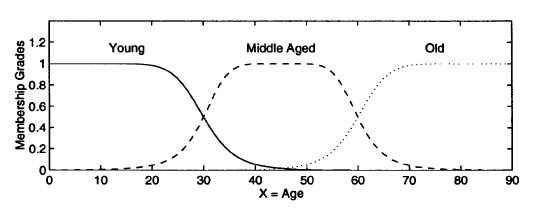
\includegraphics[width=0.8\textwidth]{./04-figuras/fund_teorica/fuzzy_sets_jang}
    \fonte{\citeonline[p.~17]{Jang1997}}
    \label{fig:fuzzy_sets_jang}
\end{figure}

Além dos conjuntos \textit{fuzzy}, há outro aspecto fundamental para o funcionamento desta lógica alternativa e poderosa: as regras \textit{fuzzy}.

%--revisao--
\subsection{Regras \textit{Fuzzy}}
\label{sec:regras_fuzzy}

As regras \textit{fuzzy} são os componentes de um sistema de inferência \textit{fuzzy} responsáveis por definir as relações entre as entradas do sistema e suas saídas e assumem a forma
\begin{center}
se $x$ é $A$ então $y$ é $B$
\end{center}
sendo ``$x$ é $A$'' denominada premissa  e ``$y$ é $B$'', consequente da regra em que $x$ e $y$ são \textit{variáveis linguísticas} de entrada e saída respectivamente  e $A$ e $B$ são os valores que elas assumem, representados por \textit{termos linguísticos}.

Uma variável linguística, segundo \citeonline[p.~54]{Jang1997}, é caracterizada por uma quíntupla $(x,T(x),X,G,M)$ em que $x$ é o nome da variável; $T(x)$ é o conjunto de termos de $x$, que é o conjunto de seus valores linguísticos ou termos linguísticos; $X$ é o universo de discurso; $G$ é uma regra sintática que gera os termos em $T(x)$; e $M$ é uma regra semântica que associa a cada termo linguístico A seu respectivo $M(A)$, em que $M(A)$ denota um conjunto \textit{fuzzy} em $X$.

Para facilitar a compreensão das definições relacionadas às variáveis linguísticas, o seguinte exemplo foi dado \cite[p.~55]{Jang1997}: se \textit{idade} é interpretado como uma variável linguística, então seu conjunto de termos $T(idade)$ poderia ser dado por:
\begin{align*}
\mbox{\textit{T(idade) = }}\{ &\mbox{ \textit{novo, não-novo, muito novo, não muito-novo,}} \dots, \\
&\mbox{ \textit{meia-idade, não de meia-idade,}} \dots, \\
&\mbox{ \textit{velho, não-velho, muito velho, mais ou menos velho, não muito velho,}} \dots, \\
&\mbox{ \textit{não muito novo e não muito velho,}} \dots \},
\end{align*}

Em que cada termo em $T(idade)$ é caracterizado por um conjunto \textit{fuzzy} de um universo de discurso $X = [0,100]$, como mostrado na Figura \ref{fig:fuzzy_rules_jang}. Geralmente, se diz ``idade é jovem'' para denotar a atribuição do valor linguístico jovem à variável linguística idade. A regra sintática se refere à forma como os valores linguísticos no conjunto de termos $T(idade)$ são gerados. A regra semântica define a função de pertinência de cada valor linguístico do conjunto de termos. A Figura \ref{fig:fuzzy_rules_jang} mostra algumas das funções de pertinência típicas para a variável linguística idade.

\begin{figure}[!htb]
    \centering
    \caption{Exemplo de função de pertinência do conjunto de termos T(idade)}
    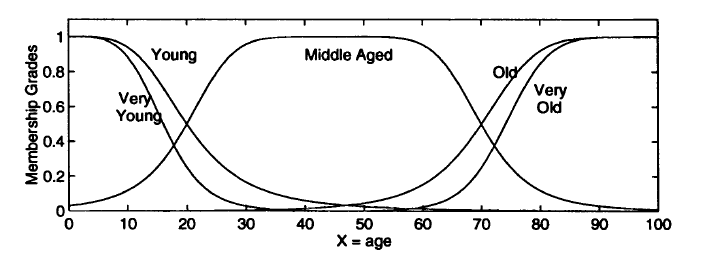
\includegraphics[width=0.8\textwidth]{./04-figuras/fund_teorica/fuzzy_rules_jang}
    \fonte{\citeonline[p.~55]{Jang1997}}
    \label{fig:fuzzy_rules_jang}
\end{figure}

Diversas regras \textit{fuzzy} fazem parte do nosso cotidiano. Exemplos possuindo a variável linguística \textit{idade} como variável linguística de entrada e saída respectivamente incluem:
\begin{center}
se \textit{idade} é \textit{jovem} então \textit{energia} é \textit{alta} \\
se \textit{sabedoria} é \textit{grande} então \textit{idade} é \textit{velha}
\end{center}

Um outro componente dos sistemas de inferência \textit{fuzzy} agrega muito valor ao uso de regras \textit{fuzzy}, permitindo a aplicação aproximada delas: o raciocínio \textit{fuzzy}.

\subsection{Raciocínio \textit{Fuzzy}}
\label{sec:raciocinio_fuzzy}

O processo de raciocínio \textit{fuzzy}, também conhecido como raciocínio aproximado, é um procedimento de inferência que deriva conclusões de um conjunto de regras \textit{fuzzy} \textit{se-então} como fatos conhecidos \cite[p.~62]{Jang1997} e é a partir dele que se pode fazer uma generalização a partir da regra básica na lógica tradicional com duas variáveis, denominada \textit{modus ponens}.

De acordo com a regra \textit{modus ponens}, podemos inferir a verdade da proposição $B$ a partir da verdade de $A$ e a implicação $A \rightarrow B$ (se A então B). Por exemplo, se $A$ é identifica por ``o tomate é vermelho'' e $B$ por ``o tomate está maduro'', então se é verdade que ``o tomate é vermelho'', é também verdade que ``o tomate está maduro''.

Contudo, o raciocínio humano emprega constantemente o modus ponens em uma maneira aproximada. Por exemplo, usando a mesma regra de implicação ``se o tomate é vermelho, então ele está maduro'', e sabemos que o ``o tomate está mais ou menos vermelho'' ($A^\prime$), então podemos inferir que ``o tomate está mais ou menos maduro'' ($B^\prime$), em que $A^\prime$ é próximo de $A$ e $B^\prime$ é próximo de $B$. Quando $A$, $B$, $A^\prime$ e $B^\prime$ são conjuntos \textit{fuzzy} do universo adequado, o procedimento de inferência descrito é chamado raciocínio aproximado ou raciocínio \textit{fuzzy}, podendo ser também chamado \textit{modus ponens} generalizado (GMP\footnote{Do inglês, \textit{Generalized Modus Ponens.}}) \cite[p.~65]{Jang1997}.

A definição formal do raciocínio aproximado (raciocínio \textit{fuzzy}) é dada por \citeonline[p.~65]{Jang1997} como: sejam $A$, $A^\prime$, e $B$ conjuntos \textit{fuzzy} de $X$, $X$ e $Y$ respectivamente; assuma que a implicação \textit{fuzzy} $A \rightarrow B$ é expressa como uma relação $R$ em $X \times Y$. Então, o conjunto \textit{fuzzy} B induzido por ``$x$ é $A$'' e a regra \textit{fuzzy} ``se $x$ é $A$ então $y$ é $B$'' é definida por:
\begin{align*}
\mu_{B^\prime}(y) &= \max\nolimits_x \min[\mu_{A^\prime}, \mu_R(x,y)]
\\
&= \vee_x[\mu_{A^\prime}(x) \wedge \mu_R(x,y)], \\
\mbox{ou, equivalentemente,} \\
B^\prime &= A^\prime \circ R = A^\prime \circ (A \rightarrow B).
\end{align*}
 
Assim, podemos usar o procedimento de inferência do raciocínio \textit{fuzzy} para derivar conclusões, dado que a implicação \textit{fuzzy} $A \rightarrow B$ é definida como uma relação \textit{fuzzy} binária apropriada.

Uma vez definidos os conjuntos, regras e raciocínio \textit{fuzzy}, pode-se mostrar como eles são utilizados em conjunto pelos sistemas de inferência \textit{fuzzy}.
 
\subsection{Sistema de Inferência \textit{Fuzzy}}
\label{sec:sistema_inferencai_fuzzy}

Um sistema de inferência fuzzy (FIS, do nome em inglês \textit{Fuzzy Inference System}) é uma ferramenta computacional popular e poderosa baseada nos conceitos de teoria de conjuntos fuzzy, regras fuzzy e raciocínio fuzzy. Há uma grande variedade de aplicações para sistemas de inferências fuzzy tais como controle automatizado, classificação de dados, análise de decisão, sistemas especialistas, predição de séries temporais, robótica e reconhecimento de padrões \cite[p.~73]{Jang1997}.

A estrutura básica de um FIS consiste de três componentes conceituais: uma base de regras, que contém uma seleção de regras fuzzy; um dicionário (ou base de dados), que define as funções de pertinência usadas nas regras fuzzy; e o mecanismo de raciocínio, que realiza o procedimento de inferência (geralmente o raciocínio fuzzy) sobre as regras e fatos dados para obter uma saída ou conclusão razoável \cite[p.~73]{Jang1997}. Sistemas de inferência fuzzy diferentes implementam estruturas ligeiramente diferentes entre si, havendo entretanto, três tipos principais de sistemas que podem ser aplicados aos mais diversos casos.

% corte 01
Os três principais tipos de FIS são os Mamdani, Tsukamoto e Sugeno e a diferença entre eles reside basicamente no consequente de suas regras fuzzy \cite[p.~74]{Jang1997}.

No sistema de inferência fuzzy Mamdani, o consequente das regras \textit{se-então} são conjuntos fuzzy. Desta forma, um sistema de inferências fuzzy Mamdani possui regras do seguinte tipo para um sistema com duas entradas e uma saída:
\begin{center}
se $x$ é $A$ e $y$ é $B$, então $z$ é $C$
\end{center}

Em que $x$, $y$ e $z$ são variáveis linguísticas nos universos de discurso $X$, $Y$ e $Z$, respectivamente e $A$, $B$ e $C$ são valores (termos) linguísticos. Com isto, um exemplo de sistema de inferências fuzzy Mamdani é formado pelas seguintes regras fuzzy:
\begin{align*}
\begin{cases}
&\mbox{Se }X  \mbox{é pequeno e } Y \mbox{é pequeno então } Z \mbox{ é muito negativo} \\
&\mbox{Se }X  \mbox{é pequeno e } Y \mbox{é grande então } Z \mbox{ é pouco negativo} \\
&\mbox{Se }X  \mbox{é grande e } Y \mbox{é pequeno então } Z \mbox{ é pouco positivo} \\
&\mbox{Se }X  \mbox{é grande e } Y \mbox{é grande então } Z \mbox{ é muito positivo} 
\end{cases}
\end{align*}

No caso do sistema de inferência fuzzy Tsukamoto, o consequente de cada regra fuzzy \textit{se-então} é representada por um conjunto fuzzy com uma função de pertinência monotônica\footnote{Uma função sempre crescente ou sempre decresente; uma função cuja derivada nunca muda de sinal}. Um exemplo de modelo fuzzy Tsukamoto de entrada única pode ser expressa como:
\begin{align*}
\begin{cases}
&\mbox{Se }X  \mbox{é pequeno então } Y \mbox{ é } C_1\\
&\mbox{Se }X  \mbox{é médio então } Y \mbox{ é } C_2\\
&\mbox{Se }X  \mbox{é grande então } Y \mbox{ é } C_3
\end{cases}
\end{align*}

No sistema de inferência fuzzy Sugeno, também conhecido como TSK (Takagi-Sugeno-Kang), o consequente é um função envolvendo as variáveis de entrada. Com isto, uma regra fuzzy típica de um modelo fuzzy Sugeno possui a seguinte forma:
\begin{center}
se $x$ é $A$ e $y$ é $B$, então $z = f(x,y)$,
\end{center}

Em que $A$ e $B$ são conjuntos fuzzy do antecedente, enquanto $z = f(x,y)$ é uma função no consequente. Geralmente, $f(x,y)$ é uma função polinomial sobre as variáveis $x$ e $y$, mas pode ser qualquer função, contanto que seja capaz de descrever apropriadamente a saída do modelo dentro da região fuzzy especificada pelo antecedente da regra. Um exemplo de sistema de inferências fuzzy TSK com duas entradas e uma saída é formado pelas seguintes regras fuzzy:
\begin{align*}
\begin{cases}
&\mbox{Se }X  \mbox{é pequeno e } Y \mbox{é pequeno então } z=-x+y+1 \\
&\mbox{Se }X  \mbox{é pequeno e } Y \mbox{é grande então } z=-y+3  \\
&\mbox{Se }X  \mbox{é grande e } Y \mbox{é pequeno então } z=-x+3  \\
&\mbox{Se }X  \mbox{é grande e } Y \mbox{é grande então } z=x+y+2  
\end{cases}
\end{align*}

Esta propriedade dos sistemas de inferência fuzzy Sugeno de possuírem, como consequente, funções paramétricas que relacionam as premissas abre várias possibilidades para sua aplicação. Uma delas é implementada por uma técnica que alia o poder das RNAs ao do FIS: o sistema de inferência neuro-fuzzy.

%Esta propriedade dos sistemas de inferência fuzzy Sugeno de possuírem, como consequente, uma função que relaciona as premissas abre várias possibilidades para sua aplicação. Uma delas é implementada por uma técnica que alia o poder de aprendizado e generalização das RNAs ao uso de variáveis linguísticas, definições de pertinência parciais e raciocínios aproximados da lógica fuzzy: o sistema de inferência neuro-fuzzy.

% corte 01
%Um sistema de inferência fuzzy pode tomar entradas fuzzy ou \textit{crisp}, mas as saídas que ele produz são sempre conjuntos fuzzy. Algumas vezes, é necessário se obter uma saída \textit{crisp}, principalmente quando o sistema de inferência fuzzy é usado como um controlador. Desta forma, se faz necessário um método de defuzzificação para extrair um valor \textit{crisp} que melhor represente um conjunto fuzzy.

%Com entradas e saídas \textit{crisp}, um sistema de inferência fuzzy implementa um mapeamento não linear do espaço de entrada para o espaço de saída. Este mapeamento é realizado por um número de regras fuzzy \textit{se-então}, cada qual descrevendo o comportamento local do mapeamento. Em particular, o antecedente de uma regra define a região fuzzy no espaço de entrada, enquanto o consequente especifica a saída na região fuzzy \cite[p.~73]{Jang1997}.